\documentclass[border=6pt]{standalone}
\usepackage{tikz}
\usetikzlibrary{arrows.meta,calc}
\begin{document}
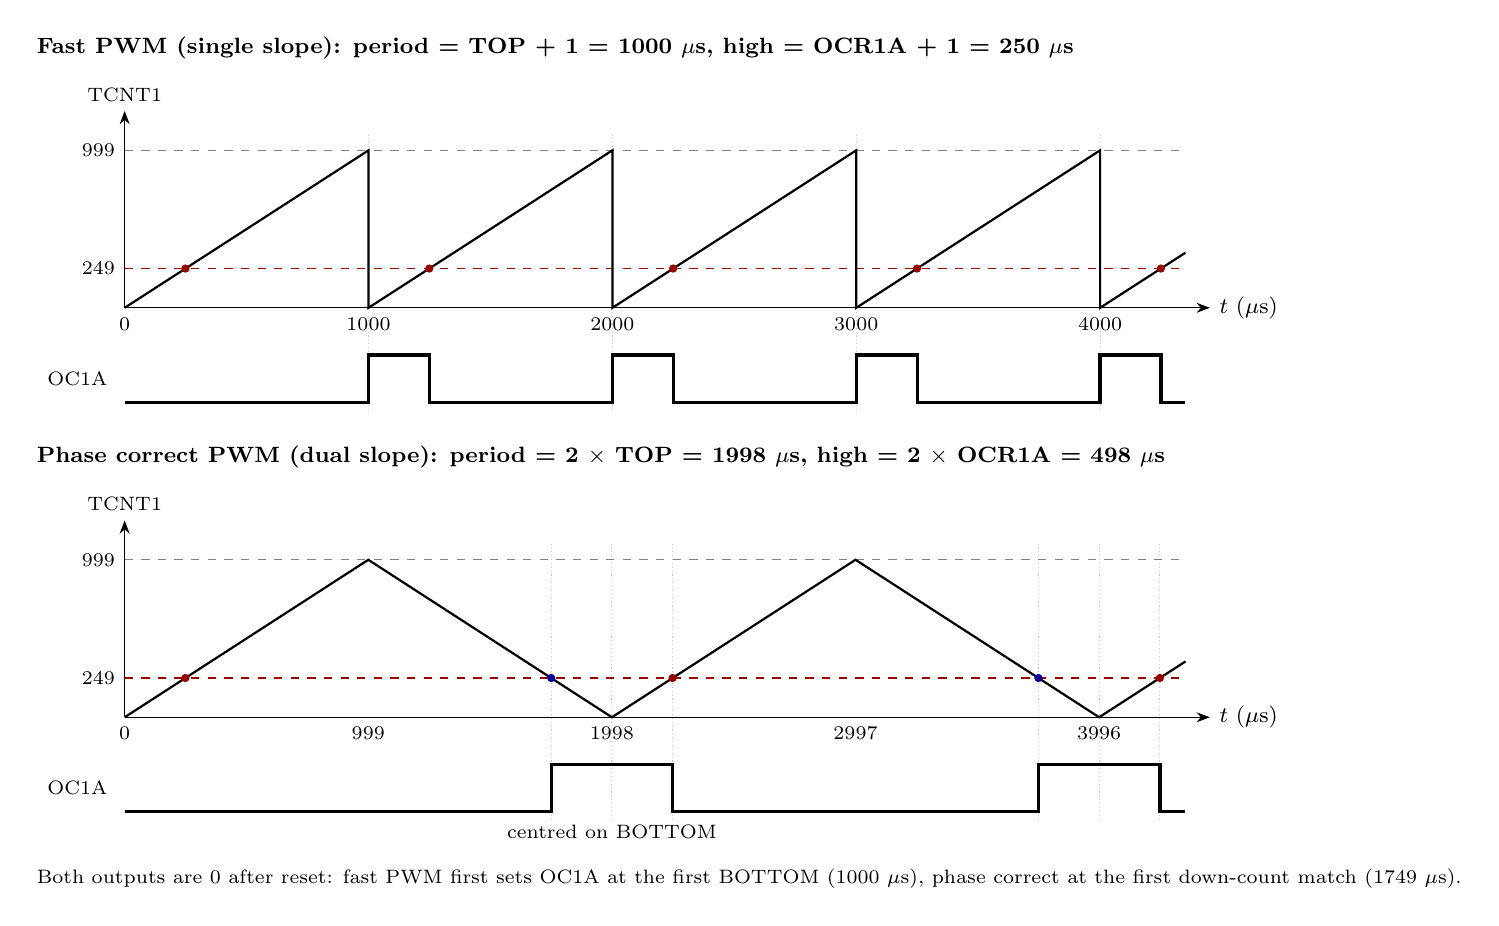
\begin{tikzpicture}[>=Stealth,font=\small,x=0.0031cm,y=1cm]
% 1 unit = 1 us; 1 MHz, no prescaler, TOP = 999, OCR1A = 249, non-inverting
\def\H{2.0}\def\C{0.4985}% 249 -> 2.0*249/999
% ---------- Fast PWM ----------
\node[font=\footnotesize\bfseries,anchor=west] at (-400,3.3) {Fast PWM (single slope): period = TOP + 1 = 1000 $\mu$s, high = OCR1A + 1 = 250 $\mu$s};
\foreach \t in {1000,2000,3000,4000} \draw[gray!45,densely dotted] (\t,-1.3) -- (\t,\H+0.2);
\draw[->] (0,0) -- (0,\H+0.5) node[above,font=\scriptsize]{TCNT1};
\draw[->] (0,0) -- (4450,0) node[right,font=\footnotesize]{$t$ ($\mu$s)};
\node[anchor=east,font=\scriptsize] at (0,\H) {999};
\node[anchor=east,font=\scriptsize] at (0,\C) {249};
\draw[gray,dashed] (0,\H) -- (4350,\H);
\draw[red!60!black,dashed] (0,\C) -- (4350,\C);
\draw[thick] (0,0) \foreach \k in {1,2,3,4} { -- (\k*1000,\H) -- (\k*1000,0) } -- (4350,{\H*0.35});
\foreach \k in {0,...,4} \fill[red!60!black] (\k*1000+249,\C) circle (1.5pt);
\foreach \t in {0,1000,2000,3000,4000} \node[below,font=\scriptsize] at (\t,0) {\t};
\begin{scope}[yshift=-1.2cm]
\node[anchor=east,font=\scriptsize] at (-30,0.3) {OC1A};
\draw[very thick] (0,0) -- (1000,0) \foreach \k in {1,2,3} { -- (\k*1000,0.6) -- (\k*1000+250,0.6) -- (\k*1000+250,0) -- (\k*1000+1000,0) } -- (4000,0.6) -- (4250,0.6) -- (4250,0) -- (4350,0);
\end{scope}
% ---------- Phase correct PWM ----------
\begin{scope}[yshift=-5.2cm]
\node[font=\footnotesize\bfseries,anchor=west] at (-400,3.3) {Phase correct PWM (dual slope): period = 2 $\times$ TOP = 1998 $\mu$s, high = 2 $\times$ OCR1A = 498 $\mu$s};
\foreach \t in {1749,1998,2247,3747,3996,4245} \draw[gray!45,densely dotted] (\t,-1.3) -- (\t,\H+0.2);
\draw[->] (0,0) -- (0,\H+0.5) node[above,font=\scriptsize]{TCNT1};
\draw[->] (0,0) -- (4450,0) node[right,font=\footnotesize]{$t$ ($\mu$s)};
\node[anchor=east,font=\scriptsize] at (0,\H) {999};
\node[anchor=east,font=\scriptsize] at (0,\C) {249};
\draw[gray,dashed] (0,\H) -- (4350,\H);
\draw[red!60!black,dashed] (0,\C) -- (4350,\C);
\draw[thick] (0,0) -- (999,\H) -- (1998,0) -- (2997,\H) -- (3996,0) -- (4350,{\H*354/999});
\foreach \t in {249,2247,4245} \fill[red!60!black] (\t,\C) circle (1.5pt);
\foreach \t in {1749,3747} \fill[blue!60!black] (\t,\C) circle (1.5pt);
\foreach \t in {0,999,1998,2997,3996} \node[below,font=\scriptsize] at (\t,0) {\t};
\begin{scope}[yshift=-1.2cm]
\node[anchor=east,font=\scriptsize] at (-30,0.3) {OC1A};
\draw[very thick] (0,0) -- (1749,0) -- (1749,0.6) -- (2247,0.6) -- (2247,0) -- (3747,0) -- (3747,0.6) -- (4245,0.6) -- (4245,0) -- (4350,0);
\node[font=\scriptsize,anchor=north] at (1998,-0.05) {centred on BOTTOM};
\end{scope}
\end{scope}
\node[font=\scriptsize,align=left,anchor=north west] at (-400,-7.0) {Both outputs are 0 after reset: fast PWM first sets OC1A at the first BOTTOM (1000 $\mu$s), phase correct at the first down-count match (1749 $\mu$s).};
\end{tikzpicture}
\end{document}
